% Options for packages loaded elsewhere
\PassOptionsToPackage{unicode}{hyperref}
\PassOptionsToPackage{hyphens}{url}
%
\documentclass[
  12pt,
]{article}
\usepackage{amsmath,amssymb}
\usepackage{iftex}
\ifPDFTeX
  \usepackage[T1]{fontenc}
  \usepackage[utf8]{inputenc}
  \usepackage{textcomp} % provide euro and other symbols
\else % if luatex or xetex
  \usepackage{unicode-math} % this also loads fontspec
  \defaultfontfeatures{Scale=MatchLowercase}
  \defaultfontfeatures[\rmfamily]{Ligatures=TeX,Scale=1}
\fi
\usepackage{lmodern}
\ifPDFTeX\else
  % xetex/luatex font selection
    \setmainfont[]{Times New Roman}
\fi
% Use upquote if available, for straight quotes in verbatim environments
\IfFileExists{upquote.sty}{\usepackage{upquote}}{}
\IfFileExists{microtype.sty}{% use microtype if available
  \usepackage[]{microtype}
  \UseMicrotypeSet[protrusion]{basicmath} % disable protrusion for tt fonts
}{}
\makeatletter
\@ifundefined{KOMAClassName}{% if non-KOMA class
  \IfFileExists{parskip.sty}{%
    \usepackage{parskip}
  }{% else
    \setlength{\parindent}{0pt}
    \setlength{\parskip}{6pt plus 2pt minus 1pt}}
}{% if KOMA class
  \KOMAoptions{parskip=half}}
\makeatother
\usepackage{xcolor}
\usepackage[margin=1in]{geometry}
\usepackage{color}
\usepackage{fancyvrb}
\newcommand{\VerbBar}{|}
\newcommand{\VERB}{\Verb[commandchars=\\\{\}]}
\DefineVerbatimEnvironment{Highlighting}{Verbatim}{commandchars=\\\{\}}
% Add ',fontsize=\small' for more characters per line
\usepackage{framed}
\definecolor{shadecolor}{RGB}{248,248,248}
\newenvironment{Shaded}{\begin{snugshade}}{\end{snugshade}}
\newcommand{\AlertTok}[1]{\textcolor[rgb]{0.94,0.16,0.16}{#1}}
\newcommand{\AnnotationTok}[1]{\textcolor[rgb]{0.56,0.35,0.01}{\textbf{\textit{#1}}}}
\newcommand{\AttributeTok}[1]{\textcolor[rgb]{0.13,0.29,0.53}{#1}}
\newcommand{\BaseNTok}[1]{\textcolor[rgb]{0.00,0.00,0.81}{#1}}
\newcommand{\BuiltInTok}[1]{#1}
\newcommand{\CharTok}[1]{\textcolor[rgb]{0.31,0.60,0.02}{#1}}
\newcommand{\CommentTok}[1]{\textcolor[rgb]{0.56,0.35,0.01}{\textit{#1}}}
\newcommand{\CommentVarTok}[1]{\textcolor[rgb]{0.56,0.35,0.01}{\textbf{\textit{#1}}}}
\newcommand{\ConstantTok}[1]{\textcolor[rgb]{0.56,0.35,0.01}{#1}}
\newcommand{\ControlFlowTok}[1]{\textcolor[rgb]{0.13,0.29,0.53}{\textbf{#1}}}
\newcommand{\DataTypeTok}[1]{\textcolor[rgb]{0.13,0.29,0.53}{#1}}
\newcommand{\DecValTok}[1]{\textcolor[rgb]{0.00,0.00,0.81}{#1}}
\newcommand{\DocumentationTok}[1]{\textcolor[rgb]{0.56,0.35,0.01}{\textbf{\textit{#1}}}}
\newcommand{\ErrorTok}[1]{\textcolor[rgb]{0.64,0.00,0.00}{\textbf{#1}}}
\newcommand{\ExtensionTok}[1]{#1}
\newcommand{\FloatTok}[1]{\textcolor[rgb]{0.00,0.00,0.81}{#1}}
\newcommand{\FunctionTok}[1]{\textcolor[rgb]{0.13,0.29,0.53}{\textbf{#1}}}
\newcommand{\ImportTok}[1]{#1}
\newcommand{\InformationTok}[1]{\textcolor[rgb]{0.56,0.35,0.01}{\textbf{\textit{#1}}}}
\newcommand{\KeywordTok}[1]{\textcolor[rgb]{0.13,0.29,0.53}{\textbf{#1}}}
\newcommand{\NormalTok}[1]{#1}
\newcommand{\OperatorTok}[1]{\textcolor[rgb]{0.81,0.36,0.00}{\textbf{#1}}}
\newcommand{\OtherTok}[1]{\textcolor[rgb]{0.56,0.35,0.01}{#1}}
\newcommand{\PreprocessorTok}[1]{\textcolor[rgb]{0.56,0.35,0.01}{\textit{#1}}}
\newcommand{\RegionMarkerTok}[1]{#1}
\newcommand{\SpecialCharTok}[1]{\textcolor[rgb]{0.81,0.36,0.00}{\textbf{#1}}}
\newcommand{\SpecialStringTok}[1]{\textcolor[rgb]{0.31,0.60,0.02}{#1}}
\newcommand{\StringTok}[1]{\textcolor[rgb]{0.31,0.60,0.02}{#1}}
\newcommand{\VariableTok}[1]{\textcolor[rgb]{0.00,0.00,0.00}{#1}}
\newcommand{\VerbatimStringTok}[1]{\textcolor[rgb]{0.31,0.60,0.02}{#1}}
\newcommand{\WarningTok}[1]{\textcolor[rgb]{0.56,0.35,0.01}{\textbf{\textit{#1}}}}
\usepackage{longtable,booktabs,array}
\usepackage{calc} % for calculating minipage widths
% Correct order of tables after \paragraph or \subparagraph
\usepackage{etoolbox}
\makeatletter
\patchcmd\longtable{\par}{\if@noskipsec\mbox{}\fi\par}{}{}
\makeatother
% Allow footnotes in longtable head/foot
\IfFileExists{footnotehyper.sty}{\usepackage{footnotehyper}}{\usepackage{footnote}}
\makesavenoteenv{longtable}
\usepackage{graphicx}
\makeatletter
\def\maxwidth{\ifdim\Gin@nat@width>\linewidth\linewidth\else\Gin@nat@width\fi}
\def\maxheight{\ifdim\Gin@nat@height>\textheight\textheight\else\Gin@nat@height\fi}
\makeatother
% Scale images if necessary, so that they will not overflow the page
% margins by default, and it is still possible to overwrite the defaults
% using explicit options in \includegraphics[width, height, ...]{}
\setkeys{Gin}{width=\maxwidth,height=\maxheight,keepaspectratio}
% Set default figure placement to htbp
\makeatletter
\def\fps@figure{htbp}
\makeatother
\setlength{\emergencystretch}{3em} % prevent overfull lines
\providecommand{\tightlist}{%
  \setlength{\itemsep}{0pt}\setlength{\parskip}{0pt}}
\setcounter{secnumdepth}{5}
% definitions for citeproc citations
\NewDocumentCommand\citeproctext{}{}
\NewDocumentCommand\citeproc{mm}{%
  \begingroup\def\citeproctext{#2}\cite{#1}\endgroup}
\makeatletter
 % allow citations to break across lines
 \let\@cite@ofmt\@firstofone
 % avoid brackets around text for \cite:
 \def\@biblabel#1{}
 \def\@cite#1#2{{#1\if@tempswa , #2\fi}}
\makeatother
\newlength{\cslhangindent}
\setlength{\cslhangindent}{1.5em}
\newlength{\csllabelwidth}
\setlength{\csllabelwidth}{3em}
\newenvironment{CSLReferences}[2] % #1 hanging-indent, #2 entry-spacing
 {\begin{list}{}{%
  \setlength{\itemindent}{0pt}
  \setlength{\leftmargin}{0pt}
  \setlength{\parsep}{0pt}
  % turn on hanging indent if param 1 is 1
  \ifodd #1
   \setlength{\leftmargin}{\cslhangindent}
   \setlength{\itemindent}{-1\cslhangindent}
  \fi
  % set entry spacing
  \setlength{\itemsep}{#2\baselineskip}}}
 {\end{list}}
\usepackage{calc}
\newcommand{\CSLBlock}[1]{\hfill\break\parbox[t]{\linewidth}{\strut\ignorespaces#1\strut}}
\newcommand{\CSLLeftMargin}[1]{\parbox[t]{\csllabelwidth}{\strut#1\strut}}
\newcommand{\CSLRightInline}[1]{\parbox[t]{\linewidth - \csllabelwidth}{\strut#1\strut}}
\newcommand{\CSLIndent}[1]{\hspace{\cslhangindent}#1}
\usepackage{tcolorbox}
\usepackage{amssymb}
\usepackage{yfonts}
\usepackage{bm}
\usepackage{titlesec}
\usepackage{kbordermatrix}


\newtcolorbox{greybox}{
  colback=white,
  colframe=blue,
  coltext=black,
  boxsep=5pt,
  arc=4pt}
  
\newcommand{\sectionbreak}{\clearpage}

 
\newcommand{\ds}[4]{\sum_{{#1}=1}^{#3}\sum_{{#2}=1}^{#4}}
\newcommand{\us}[3]{\mathop{\sum\sum}_{1\leq{#2}<{#1}\leq{#3}}}

\newcommand{\ol}[1]{\overline{#1}}
\newcommand{\ul}[1]{\underline{#1}}

\newcommand{\amin}[1]{\mathop{\text{argmin}}_{#1}}
\newcommand{\amax}[1]{\mathop{\text{argmax}}_{#1}}

\newcommand{\ci}{\perp\!\!\!\perp}

\newcommand{\mc}[1]{\mathcal{#1}}
\newcommand{\mb}[1]{\mathbb{#1}}
\newcommand{\mf}[1]{\mathfrak{#1}}

\newcommand{\eps}{\epsilon}
\newcommand{\lbd}{\lambda}
\newcommand{\alp}{\alpha}
\newcommand{\df}{=:}
\newcommand{\am}[1]{\mathop{\text{argmin}}_{#1}}
\newcommand{\ls}[2]{\mathop{\sum\sum}_{#1}^{#2}}
\newcommand{\ijs}{\mathop{\sum\sum}_{1\leq i<j\leq n}}
\newcommand{\jis}{\mathop{\sum\sum}_{1\leq j<i\leq n}}
\newcommand{\sij}{\sum_{i=1}^n\sum_{j=1}^n}
	
\ifLuaTeX
  \usepackage{selnolig}  % disable illegal ligatures
\fi
\usepackage{bookmark}
\IfFileExists{xurl.sty}{\usepackage{xurl}}{} % add URL line breaks if available
\urlstyle{same}
\hypersetup{
  pdfauthor={Jan de Leeuw - University of California Los Angeles},
  hidelinks,
  pdfcreator={LaTeX via pandoc}}

\title{Smacof at 50: A Manual\\
Part 4: smacofRO - Non-metric Smacof for Rank Order Data}
\author{Jan de Leeuw - University of California Los Angeles}
\date{Started May 12 2024, Version of May 20, 2024}

\begin{document}
\maketitle

{
\setcounter{tocdepth}{3}
\tableofcontents
}
\textbf{Note:} This is a working manuscript which will be expanded/updated
frequently. All suggestions for improvement are welcome. All Rmd, tex,
html, pdf, R, and C files are in the public domain. Attribution will be
appreciated, but is not required. The files can be found at
\url{https://github.com/deleeuw} in the smacofRO directories of the
repositories smacofCode, smacofManual, and smacofExamples.

\section{Introduction}\label{introduction}

The smacofRO program is a non-metric MDS program designed
to handle a partial order over dissimilarities of pairs of objects selected
from a single set. In the terminology of Coombs (1964) we are dealing
with QIVa similarity data. Typically the partial order is derived from a
symmetric numerical matrix of dissimilarities or from a ranking
(with or without ties) of the dissimilarities.

\subsection{Parameters}\label{parameters}

The smacofRO function in R has the following parameters (with default values).

\begin{Shaded}
\begin{Highlighting}[]
\NormalTok{smacofRO }\OtherTok{\textless{}{-}} \ControlFlowTok{function}\NormalTok{(data,}
\NormalTok{                     ndim,}
                     \AttributeTok{xold =} \ConstantTok{NULL}\NormalTok{,}
                     \AttributeTok{labels =} \ConstantTok{NULL}\NormalTok{,}
                     \AttributeTok{width =} \DecValTok{15}\NormalTok{,}
                     \AttributeTok{precision =} \DecValTok{10}\NormalTok{,}
                     \AttributeTok{itmax =} \DecValTok{1000}\NormalTok{,}
                     \AttributeTok{eps =} \FloatTok{1e{-}10}\NormalTok{,}
                     \AttributeTok{verbose =} \ConstantTok{TRUE}\NormalTok{,}
                     \AttributeTok{kitmax =} \DecValTok{5}\NormalTok{,}
                     \AttributeTok{keps =} \FloatTok{1e{-}10}\NormalTok{,}
                     \AttributeTok{kverbose =} \ConstantTok{FALSE}\NormalTok{,}
                     \AttributeTok{init =} \DecValTok{1}\NormalTok{,}
                     \AttributeTok{ties =} \DecValTok{1}\NormalTok{)}
\end{Highlighting}
\end{Shaded}

\begin{itemize}
\tightlist
\item
  If xold is non-null then an initial configuration matrix must be provided.
\item
  If labels is non-null then a character vector of plot labels must be provided.
\item
  width and precision are relevant for the format of (optional) major iteration output.
\item
  itmax and eps determine when the major iterations stop.
\item
  If verbose = TRUE itel and stress for each major iteration are
  written to stdout.
\item
  kitmax and keps determine the number of inner Guttman transform iterations
  between two monotone regressions.
\item
  If kverbose = TRUE then itel and stress for each inner iteration are written to stdout.
\item
  If init = 1 the Torgerson initial configuration is computed, if init = 2
  the maximum sum initial configuration is used, if init = 3 a random initial configuration
  is used.
\item
  Ties is either 1, 2, or 3 indicating if the primary, secondary, or tertiary
  apprach to ties should be used.
\end{itemize}

\subsection{Input}\label{input}

The data are entered in a five-column table. Here are the first five rows for
the Gruijter example, analyzed below.

\begin{Shaded}
\begin{Highlighting}[]
\NormalTok{     i j delta     weight ties}
\NormalTok{[}\DecValTok{1}\NormalTok{,] }\DecValTok{7} \DecValTok{6}  \FloatTok{3.20} \FloatTok{0.02777778}    \DecValTok{1}
\NormalTok{[}\DecValTok{2}\NormalTok{,] }\DecValTok{2} \DecValTok{1}  \FloatTok{4.08} \FloatTok{0.02777778}    \DecValTok{2}
\NormalTok{[}\DecValTok{3}\NormalTok{,] }\DecValTok{3} \DecValTok{2}  \FloatTok{4.59} \FloatTok{0.02777778}    \DecValTok{3}
\NormalTok{[}\DecValTok{4}\NormalTok{,] }\DecValTok{6} \DecValTok{5}  \FloatTok{4.60} \FloatTok{0.02777778}    \DecValTok{4}
\NormalTok{[}\DecValTok{5}\NormalTok{,] }\DecValTok{8} \DecValTok{4}  \FloatTok{4.67} \FloatTok{0.02777778}    \DecValTok{5}
\end{Highlighting}
\end{Shaded}

The first two columns of data give the indices of the dissimilarities. Always \(1\leq j<i\leq n\).
Column three gives the value of delta, which can be an observed numerical value or
a rank number. The data are in non-increasing order within their
column. Column four gives the weights, adding up to one over all observations.
And the last column codes tieblocks. Data is allowed to have are fewer than \(\frac12n(n-1)\) rows,
but each index pair should occur at most one time.
Missing pairs are computationally equivalent to rows with weight equal to zero.

Typically we create the data by using the utility function smacofMakeRankOrderData(), which is part of the
smacofRO package.

\begin{Shaded}
\begin{Highlighting}[]
\NormalTok{smacofMakeRankOrderData }\OtherTok{\textless{}{-}}
  \ControlFlowTok{function}\NormalTok{(delta, }\AttributeTok{weights =} \ConstantTok{NULL}\NormalTok{, }\AttributeTok{tieblocks =} \ConstantTok{TRUE}\NormalTok{)}
\end{Highlighting}
\end{Shaded}

Here delta is a symmetric matrix or an object of class dist containing the dissimilarities.
If weights is NULL all weights are assumed to be equal.

\subsection{Algorithm}\label{algorithm}

\begin{itemize}
\tightlist
\item
  The ALS algorithm alternates a number of inner Guttman iterations with a single monotone
  regression (with one of the three options for ties, cf De Leeuw (1977)).
\item
  The maximum number of inner iterations is kitmax, if the stress in an
  inner iteration changes less than keps the inner iterations are also stopped.
\item
  Guttman iterations are normalized explicitly, using \(\sum\sum w_{ij}d_{ij}^2(X)=1\).
\item
  The maximum number of outer iterations is itmax, if the stress in an
  outer iteration changes less than eps the outer iterations are also stopped.
\item
  For monotone regression we use the pava algorithm from De Leeuw (2017), with
  some additional code for the tertiary approach to ties.
\end{itemize}

\subsection{Output}\label{output}

The program returns a list with the following elements.

\begin{Shaded}
\begin{Highlighting}[]
\NormalTok{  h }\OtherTok{\textless{}{-}} \FunctionTok{list}\NormalTok{(}
    \AttributeTok{nobj =}\NormalTok{ nobj,}
    \AttributeTok{ndim =}\NormalTok{ ndim,}
    \AttributeTok{snew =}\NormalTok{ snew,}
    \AttributeTok{itel =}\NormalTok{ itel,}
    \AttributeTok{xnew =}\NormalTok{ xnew,}
    \AttributeTok{delta =}\NormalTok{ delta,}
    \AttributeTok{evec =}\NormalTok{ evec,}
    \AttributeTok{dvec =}\NormalTok{ dvec,}
    \AttributeTok{wvec =}\NormalTok{ wvec,}
    \AttributeTok{labels =}\NormalTok{ labels}
\NormalTok{  )}
\end{Highlighting}
\end{Shaded}

\begin{itemize}
\tightlist
\item
  nobj is the number of objects.
\item
  ndim is the number of dimensions.
\item
  snew is the final value of stress.
\item
  itel is the number of major iterations.
\item
  xnew is a matrix with the final configuration.
\item
  delta is a vector with the dissimilarities.
\item
  wvec is a vector with the weights.
\item
  evec is a vector with the final disparities.
\item
  dvec is a vector with the final distances.
\item
  labels is the character vector of labels (or NULL).
\end{itemize}

The elements of delta, wvec, evec, and dvec are all in the order of the
input data, i.e.~sorted by increasing delta.

\subsection{Plots}\label{plots}

The output list of smacofRO can be passed to the three utility programs that make plots.
In addition to the list with smacofRO output the plot functions have a number of the
standard graphical parameters. smacofConfigurationPlot() uses labels (if available) to label the
points. The fitlines argument of smacofShepardPlot() and smacofDistDhatplot()
connects pairs of points in the plot that coincide if stress is zero. The sum of the squared lengths
of the fitlines is equal to the stress.

\begin{Shaded}
\begin{Highlighting}[]
\NormalTok{smacofShepardPlot }\OtherTok{\textless{}{-}}
  \ControlFlowTok{function}\NormalTok{(h,}
           \AttributeTok{main =} \StringTok{"ShepardPlot"}\NormalTok{,}
           \AttributeTok{fitlines =} \ConstantTok{TRUE}\NormalTok{,}
           \AttributeTok{colline =} \StringTok{"RED"}\NormalTok{,}
           \AttributeTok{colpoint =} \StringTok{"BLUE"}\NormalTok{,}
           \AttributeTok{resolution =} \DecValTok{100}\NormalTok{,}
           \AttributeTok{lwd =} \DecValTok{2}\NormalTok{,}
           \AttributeTok{cex =} \DecValTok{1}\NormalTok{,}
           \AttributeTok{pch =} \DecValTok{16}\NormalTok{)}
           
\NormalTok{smacofConfigurationPlot }\OtherTok{\textless{}{-}}
  \ControlFlowTok{function}\NormalTok{(h,}
           \AttributeTok{main =} \StringTok{"ConfigurationPlot"}\NormalTok{,}
           \AttributeTok{dim1 =} \DecValTok{1}\NormalTok{,}
           \AttributeTok{dim2 =} \DecValTok{2}\NormalTok{,}
           \AttributeTok{pch =} \DecValTok{16}\NormalTok{,}
           \AttributeTok{col =} \StringTok{"RED"}\NormalTok{,}
           \AttributeTok{cex =} \FloatTok{1.5}\NormalTok{)}
           
\NormalTok{smacofDistDhatPlot }\OtherTok{\textless{}{-}} \ControlFlowTok{function}\NormalTok{(h,}
                               \AttributeTok{fitlines =} \ConstantTok{TRUE}\NormalTok{,}
                               \AttributeTok{colline =} \StringTok{"RED"}\NormalTok{,}
                               \AttributeTok{colpoint =} \StringTok{"BLUE"}\NormalTok{,}
                               \AttributeTok{main =} \StringTok{"Dist{-}Dhat Plot"}\NormalTok{,}
                               \AttributeTok{cex =} \DecValTok{1}\NormalTok{,}
                               \AttributeTok{lwd =} \DecValTok{2}\NormalTok{,}
                               \AttributeTok{pch =} \DecValTok{16}\NormalTok{)}
\end{Highlighting}
\end{Shaded}

\section{Examples}\label{examples}

\subsection{De Gruijter (1967)}\label{degruijter_67}

In this example the number of tieblocks is 35, which means
there is only a single tieblock of two observations, the other 34 observations are
untied. We expect that the three different ways of handling ties will not make
much of a difference.

\begin{Shaded}
\begin{Highlighting}[]
\NormalTok{h1 }\OtherTok{\textless{}{-}} \FunctionTok{smacofRO}\NormalTok{(gruijterData, }\DecValTok{2}\NormalTok{, }\AttributeTok{ties =} \DecValTok{1}\NormalTok{, }\AttributeTok{labels =}\NormalTok{ labels, }\AttributeTok{verbose =} \ConstantTok{FALSE}\NormalTok{)}
\NormalTok{h2 }\OtherTok{\textless{}{-}} \FunctionTok{smacofRO}\NormalTok{(gruijterData, }\DecValTok{2}\NormalTok{, }\AttributeTok{ties =} \DecValTok{2}\NormalTok{, }\AttributeTok{labels =}\NormalTok{ labels, }\AttributeTok{verbose =} \ConstantTok{FALSE}\NormalTok{)}
\NormalTok{h3 }\OtherTok{\textless{}{-}} \FunctionTok{smacofRO}\NormalTok{(gruijterData, }\DecValTok{2}\NormalTok{, }\AttributeTok{ties =} \DecValTok{3}\NormalTok{, }\AttributeTok{labels =}\NormalTok{ labels, }\AttributeTok{verbose =} \ConstantTok{FALSE}\NormalTok{)}
\end{Highlighting}
\end{Shaded}

\begin{itemize}
\tightlist
\item
  Ties = 1 uses 88 iterations and stops at stress 0.0042180140
\item
  Ties = 2 uses 65 iterations and stops at stress 0.0042573281
\item
  Ties = 3 uses 69 iterations and stops at stress 0.0040850898
\end{itemize}

And indeed the solutions are practically the same, although the number of iterations needed for convergence
differs somewhat between options. We only show one Shepardplot, because the other two are virtually the same.

\begin{center}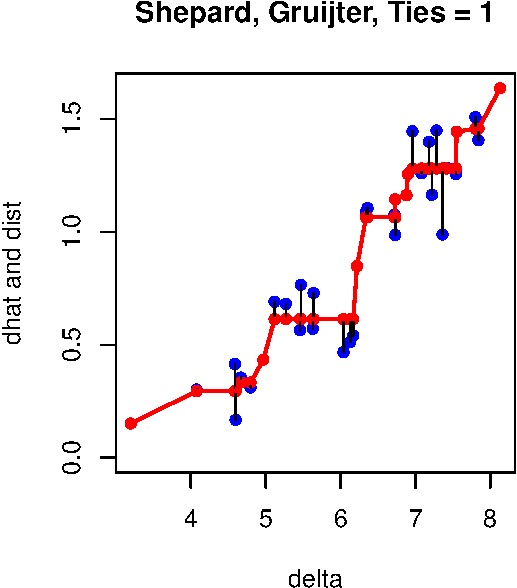
\includegraphics{smacofRO_files/figure-latex/plotgruijter-1} \end{center}

We can also use this example to show the effect of using different initial configurations.

\begin{Shaded}
\begin{Highlighting}[]
\NormalTok{h1 }\OtherTok{\textless{}{-}} \FunctionTok{smacofRO}\NormalTok{(gruijterData, }\DecValTok{2}\NormalTok{, }\AttributeTok{init =} \DecValTok{1}\NormalTok{, }\AttributeTok{labels =}\NormalTok{ labels, }\AttributeTok{verbose =} \ConstantTok{FALSE}\NormalTok{)}
\NormalTok{h2 }\OtherTok{\textless{}{-}} \FunctionTok{smacofRO}\NormalTok{(gruijterData, }\DecValTok{2}\NormalTok{, }\AttributeTok{init =} \DecValTok{2}\NormalTok{, }\AttributeTok{labels =}\NormalTok{ labels, }\AttributeTok{verbose =} \ConstantTok{FALSE}\NormalTok{)}
\NormalTok{h3 }\OtherTok{\textless{}{-}} \FunctionTok{smacofRO}\NormalTok{(gruijterData, }\DecValTok{2}\NormalTok{, }\AttributeTok{init =} \DecValTok{3}\NormalTok{, }\AttributeTok{labels =}\NormalTok{ labels, }\AttributeTok{verbose =} \ConstantTok{FALSE}\NormalTok{)}
\end{Highlighting}
\end{Shaded}

\begin{itemize}
\tightlist
\item
  Init = 1 uses 88 iterations and stops at stress 0.0042180140
\item
  Init = 2 uses 76 iterations and stops at stress 0.0039894695
\item
  Init = 3 uses 69 iterations and stops at stress 0.0060410599
\end{itemize}

\begin{center}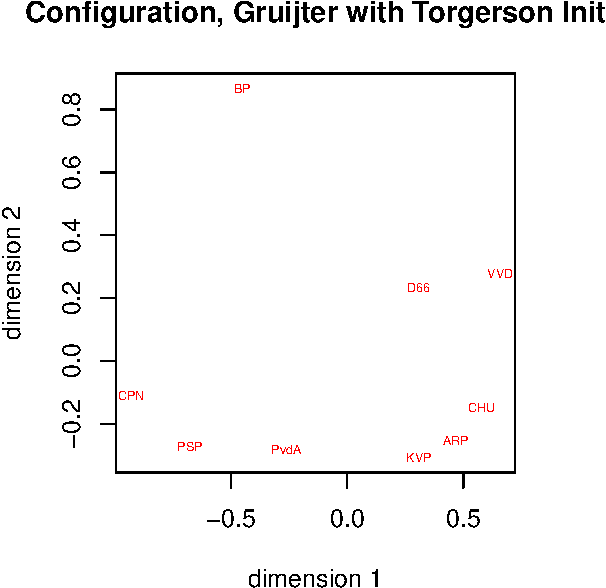
\includegraphics{smacofRO_files/figure-latex/gruiterconfs-1} \end{center}

\begin{center}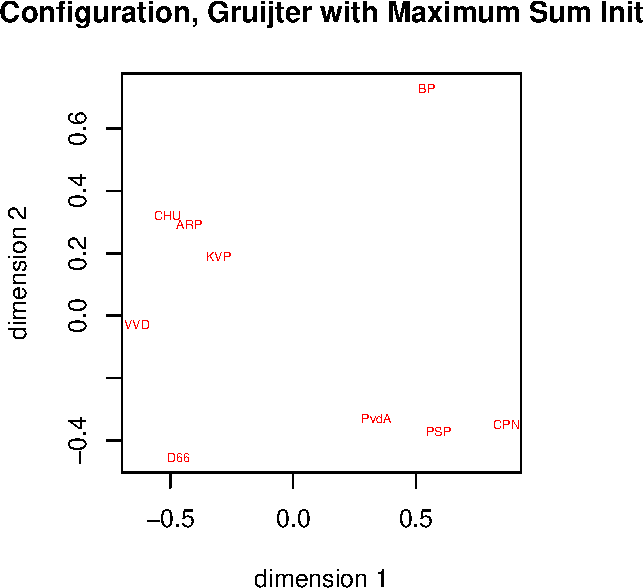
\includegraphics{smacofRO_files/figure-latex/gruiterconfs-2} \end{center}

\begin{center}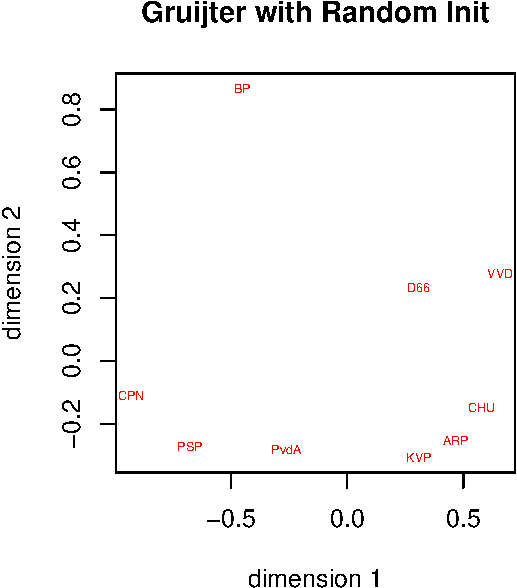
\includegraphics{smacofRO_files/figure-latex/gruiterconfs-3} \end{center}

Using different initial configurations in this example makes a huge difference. All three plots
show the (CPN, PvdA, PSP) leftist cluster, the liberal (VVD, D'66) cluster, the protest BP outlier which is its own cluster, and the (KVP, ARP, CHU) christian democrat cluster. But in the three plots the
clusters are distributed quite differently over the plane.

\subsection{Ekman (1954)}\label{ekman_54}

In the Ekman data there are 47 tieblocks out of
91 observations, and we expect the
ties option to make some difference.

\begin{Shaded}
\begin{Highlighting}[]
\NormalTok{h1 }\OtherTok{\textless{}{-}} \FunctionTok{smacofRO}\NormalTok{(ekmanData, }\DecValTok{2}\NormalTok{, }\AttributeTok{ties =} \DecValTok{1}\NormalTok{, }\AttributeTok{verbose =} \ConstantTok{FALSE}\NormalTok{, }\AttributeTok{labels =}\NormalTok{ labels, }\AttributeTok{itmax =} \DecValTok{10000}\NormalTok{)}
\NormalTok{h2 }\OtherTok{\textless{}{-}} \FunctionTok{smacofRO}\NormalTok{(ekmanData, }\DecValTok{2}\NormalTok{, }\AttributeTok{ties =} \DecValTok{2}\NormalTok{, }\AttributeTok{verbose =} \ConstantTok{FALSE}\NormalTok{, }\AttributeTok{labels =}\NormalTok{ labels, }\AttributeTok{itmax =} \DecValTok{10000}\NormalTok{)}
\NormalTok{h3 }\OtherTok{\textless{}{-}} \FunctionTok{smacofRO}\NormalTok{(ekmanData, }\DecValTok{2}\NormalTok{, }\AttributeTok{ties =} \DecValTok{3}\NormalTok{, }\AttributeTok{verbose =} \ConstantTok{FALSE}\NormalTok{, }\AttributeTok{labels =}\NormalTok{ labels, }\AttributeTok{itmax =} \DecValTok{10000}\NormalTok{)}
\end{Highlighting}
\end{Shaded}

\begin{itemize}
\tightlist
\item
  Ties = 1 uses 40 iterations and stops at stress 0.0002668633
\item
  Ties = 2 uses 32 iterations and stops at stress 0.0004988332
\item
  Ties = 3 uses 1400 iterations and stops at stress 0.0000000320
\end{itemize}

Although the stress values are indeed different the solutions for ties = 1 and ties = 2 are very similar.
Also note that for ties = 3 a huge number of iterations is needed to
bring stress very close to zero, indicating perfect fit and very slow, and possibly sublinear, convergence.
Remember that for ties = 3 there is only stress between tieblocks, no stress within tieblocks.

We now look at the Shepard plots and the configuration plots.

\begin{center}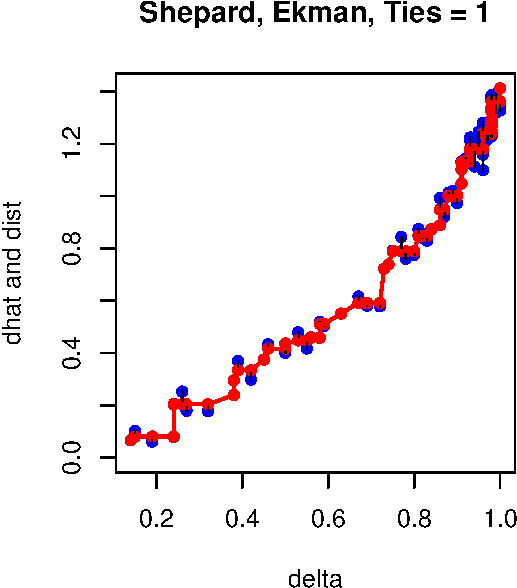
\includegraphics{smacofRO_files/figure-latex/plotekman-1} \end{center}

\begin{center}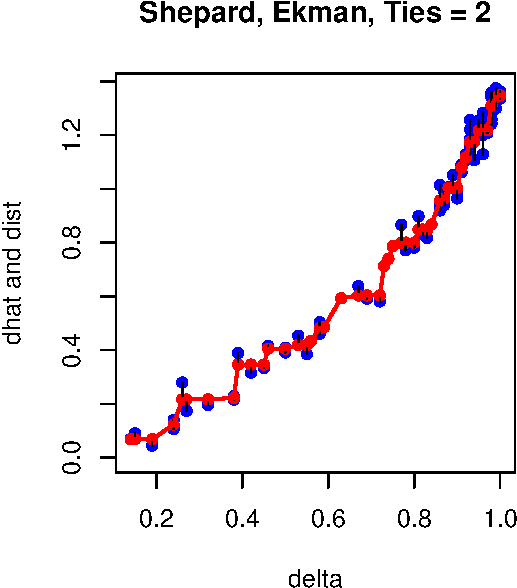
\includegraphics{smacofRO_files/figure-latex/plotekman-2} \end{center}

\begin{center}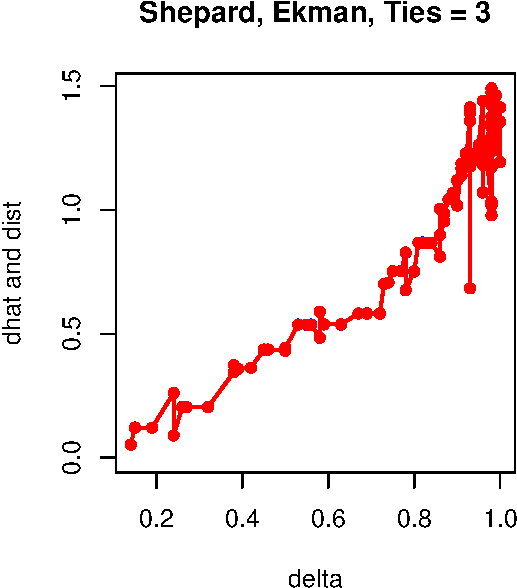
\includegraphics{smacofRO_files/figure-latex/plotekman-3} \end{center}

When looking at the
Shepard plots we have to remember that for ties = 1 and ties = 3 we can have different disparity values for the
same dissimilarity value. Thus tieblocks are represented as intervals on the vertical axis, and strictly spoken we do not have a functional relationship between delta and dhat. This is clear from the plot for the
tertiary approach, which shows some of the intervals, mostly for the larger dissimilarities. It reinforces the
idea that the tertiary approach is mostly useful if there are many small tieblocks, in which case it will be quite similar to the primary and secondary approach.

If we compare the three Shepard plots we see that ties = 1 and ties = 2 are very similar, but ties = 3
is different. There are no blue points in the plot for ties = 3, for the simple reason that they are
identical to the red points. The stress is practically zero, which means that smacof is able to scale
the 47 tieblock averages in the correct order. Plots for ties = 1 and ties = 2
show the black fitlines, which indicate less than perfect fit. There are no fitlines in the plot for ties = 3.

\begin{center}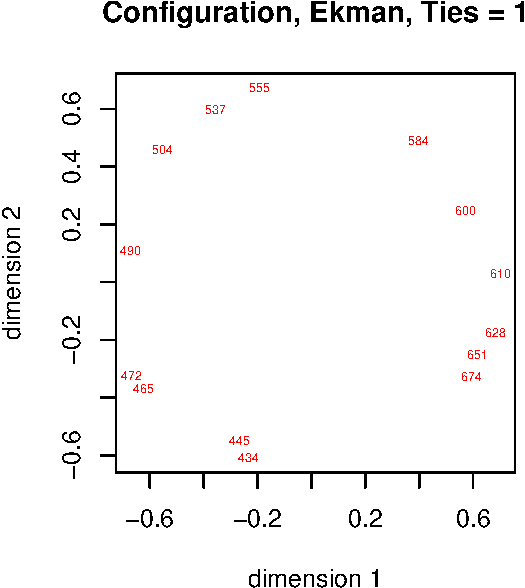
\includegraphics{smacofRO_files/figure-latex/plotekmanconfs-1} \end{center}

\begin{center}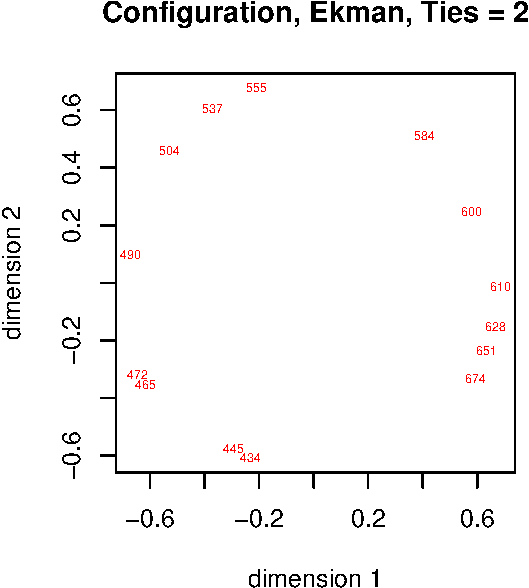
\includegraphics{smacofRO_files/figure-latex/plotekmanconfs-2} \end{center}

\begin{center}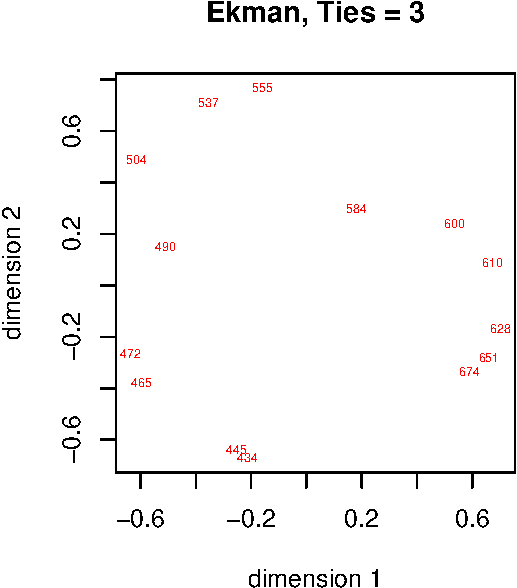
\includegraphics{smacofRO_files/figure-latex/plotekmanconfs-3} \end{center}

In configuration plots for ties = 1 and ties = 2 are very similar, and they show
the color circle in all its glory. For ties = 3 the circle has some serious dents,
which are presumably needed to force stress to zero.

For completeness we also give the dist-dhat plots corresponding with the
three ties options. They again show the perfect fit with ties = 3 and the
similarity of the fits for ties = 1 and ties = 2.

\begin{center}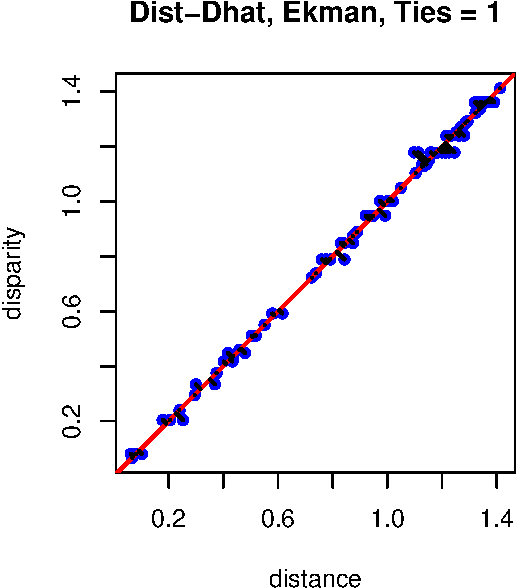
\includegraphics{smacofRO_files/figure-latex/plotekmandd-1} \end{center}

\begin{center}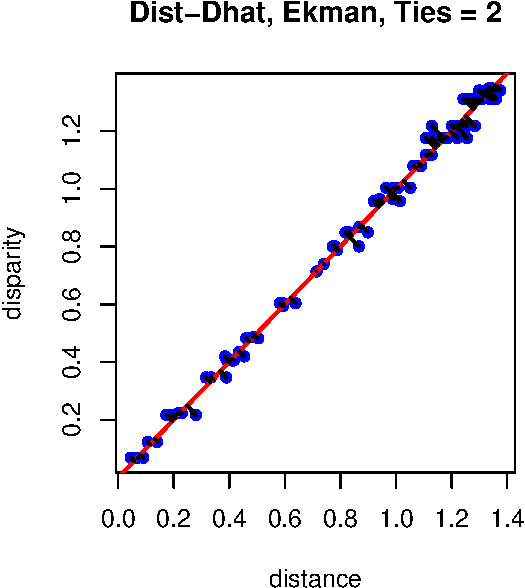
\includegraphics{smacofRO_files/figure-latex/plotekmandd-2} \end{center}

\begin{center}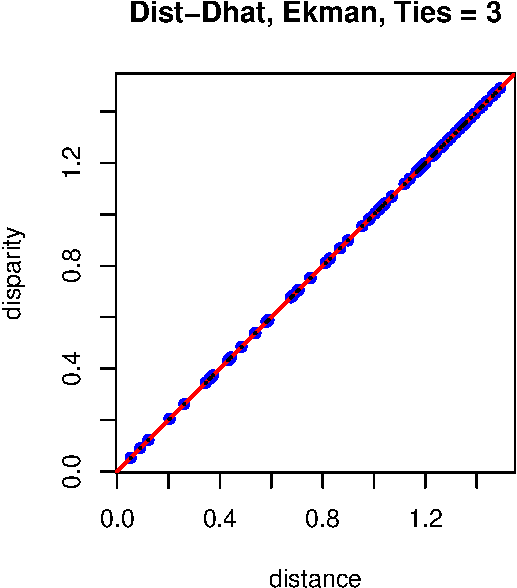
\includegraphics{smacofRO_files/figure-latex/plotekmandd-3} \end{center}

\subsection{Rothkopf (1957)}\label{rothkopf_57}

In the morse code data there are 68 tieblocks out of
630 observations. Thus almost all observations are tied.

\begin{Shaded}
\begin{Highlighting}[]
\NormalTok{h1 }\OtherTok{\textless{}{-}} \FunctionTok{smacofRO}\NormalTok{(morseData, }\DecValTok{2}\NormalTok{, }\AttributeTok{ties =} \DecValTok{1}\NormalTok{, }\AttributeTok{verbose =} \ConstantTok{FALSE}\NormalTok{, }\AttributeTok{itmax =} \DecValTok{10000}\NormalTok{, }\AttributeTok{labels =}\NormalTok{ labels)}
\NormalTok{h2 }\OtherTok{\textless{}{-}} \FunctionTok{smacofRO}\NormalTok{(morseData, }\DecValTok{2}\NormalTok{, }\AttributeTok{ties =} \DecValTok{2}\NormalTok{, }\AttributeTok{verbose =} \ConstantTok{FALSE}\NormalTok{, }\AttributeTok{itmax =} \DecValTok{10000}\NormalTok{, }\AttributeTok{labels =}\NormalTok{ labels)}
\NormalTok{h3 }\OtherTok{\textless{}{-}} \FunctionTok{smacofRO}\NormalTok{(morseData, }\DecValTok{2}\NormalTok{, }\AttributeTok{ties =} \DecValTok{3}\NormalTok{, }\AttributeTok{verbose =} \ConstantTok{FALSE}\NormalTok{, }\AttributeTok{itmax =} \DecValTok{10000}\NormalTok{, }\AttributeTok{labels =}\NormalTok{ labels)}
\end{Highlighting}
\end{Shaded}

\begin{itemize}
\tightlist
\item
  Ties = 1 uses 34 iterations and stops at stress 0.0163278414
\item
  Ties = 2 uses 30 iterations and stops at stress 0.0203202336
\item
  Ties = 3 uses 1129 iterations and stops at stress 0.0000000226
\end{itemize}

\begin{center}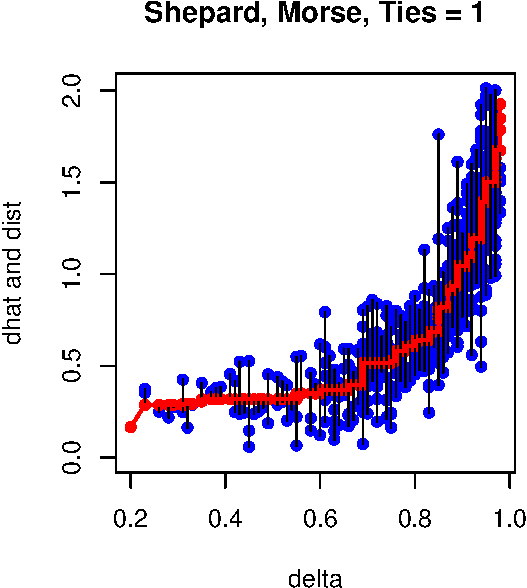
\includegraphics{smacofRO_files/figure-latex/plotmorse-1} \end{center}

\begin{center}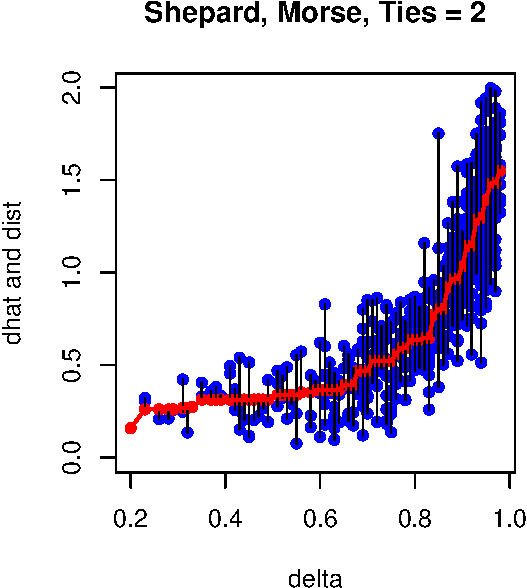
\includegraphics{smacofRO_files/figure-latex/plotmorse-2} \end{center}

\begin{center}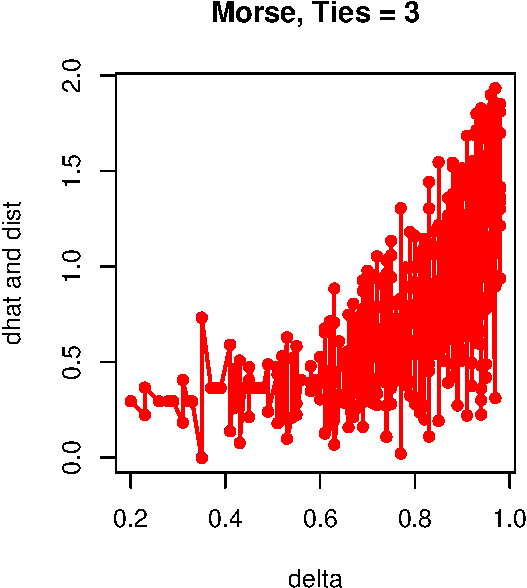
\includegraphics{smacofRO_files/figure-latex/plotmorse-3} \end{center}

We see the same types of results in the iterations and the Shepard plots as before. For ties = 3
stress is again close to zero and we require a huge number of iterations. The Shepard plot
for ties = 3 is messy, because there are so many intervals and intervals can be wide because
within tieblocks there is no stress.

\begin{center}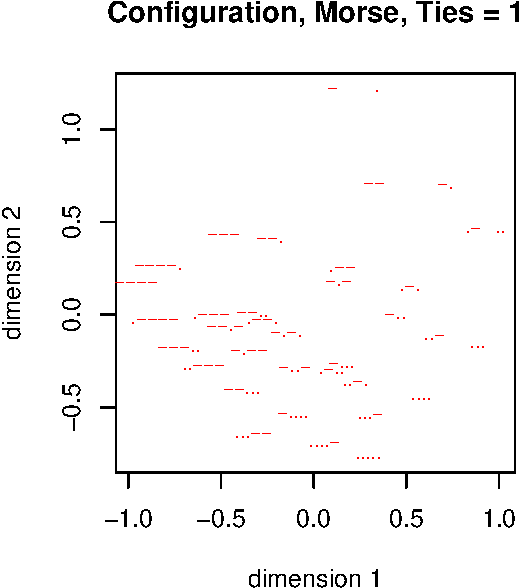
\includegraphics{smacofRO_files/figure-latex/plotmorseconfs-1} \end{center}

\begin{center}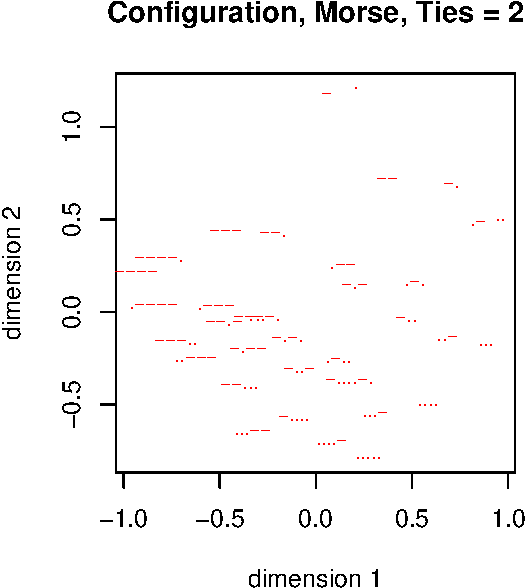
\includegraphics{smacofRO_files/figure-latex/plotmorseconfs-2} \end{center}

\begin{center}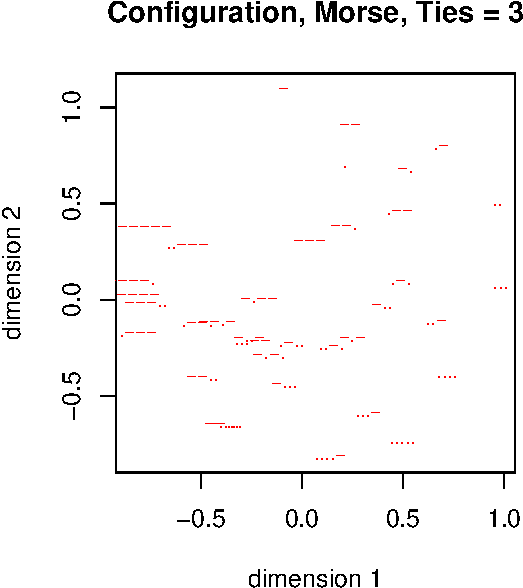
\includegraphics{smacofRO_files/figure-latex/plotmorseconfs-3} \end{center}

Configuration plots for ties = 1 and ties = 2 are similar and show parallel lines for morse codes
with one, two, three, four, or five symbols. On those five parallel lines codes are ordered from
all dashes to all dots. For ties = 3 that nice raster structure is again disturbed.

We also run morse with different values of kitmax, the number of inner Guttman iterations. The results are

\begin{Shaded}
\begin{Highlighting}[]
\NormalTok{h1 }\OtherTok{\textless{}{-}} \FunctionTok{smacofRO}\NormalTok{(morseData, }\DecValTok{2}\NormalTok{, }\AttributeTok{kitmax =} \DecValTok{1}\NormalTok{, }\AttributeTok{verbose =} \ConstantTok{FALSE}\NormalTok{, }\AttributeTok{itmax =} \DecValTok{10000}\NormalTok{)}
\NormalTok{h2 }\OtherTok{\textless{}{-}} \FunctionTok{smacofRO}\NormalTok{(morseData, }\DecValTok{2}\NormalTok{, }\AttributeTok{kitmax =} \DecValTok{5}\NormalTok{, }\AttributeTok{verbose =} \ConstantTok{FALSE}\NormalTok{, }\AttributeTok{itmax =} \DecValTok{10000}\NormalTok{)}
\NormalTok{h3 }\OtherTok{\textless{}{-}} \FunctionTok{smacofRO}\NormalTok{(morseData, }\DecValTok{2}\NormalTok{, }\AttributeTok{kitmax =} \DecValTok{10}\NormalTok{, }\AttributeTok{verbose =} \ConstantTok{FALSE}\NormalTok{, }\AttributeTok{itmax =} \DecValTok{10000}\NormalTok{)}
\end{Highlighting}
\end{Shaded}

\begin{itemize}
\tightlist
\item
  Kitmax = 1 uses 138 major iterations and stops at stress 0.0163278417
\item
  Kitmax = 5 uses 34 major iterations and stops at stress 0.0163278414
\item
  Kitmax = 10 uses 22 major iterations and stops at stress 0.0163278414
\end{itemize}

We see that the resulting stress values are pretty much the same, but the number of outer iterations differs. This may be significant, because it means that using only one Guttman iteration means doing 138 monotone
regressions, while having ten Guttman iterations per major iteration only uses 22 monotone
regressions. On the other hand for kitmax 1, 5, 10 we have to do respectively 138, 170, and 220 inner Guttman iterations. Which of the three options is faster will depend on the relative time required by Guttman transforms
and monotone regressions. The timing for the current implementation, with 100 replications in microbenchmark
(Mersmann (2023)), is as follows.

\begin{verbatim}
## Warning in microbenchmark(smacofRO(morseData, 2, kitmax = 1, verbose = FALSE, :
## less accurate nanosecond times to avoid potential integer overflows
\end{verbatim}

\begin{verbatim}
## Unit: milliseconds
##                                                                 expr       min
##   smacofRO(morseData, 2, kitmax = 1, verbose = FALSE, itmax = 10000) 1336.8770
##   smacofRO(morseData, 2, kitmax = 5, verbose = FALSE, itmax = 10000)  484.2788
##  smacofRO(morseData, 2, kitmax = 10, verbose = FALSE, itmax = 10000)  418.8768
##         lq      mean    median        uq       max neval
##  1360.1857 1372.0015 1368.2405 1379.6018 1506.5266   100
##   494.0313  498.0338  496.7758  500.0796  538.6924   100
##   429.6171  434.6207  432.5188  437.1846  454.1709   100
\end{verbatim}

It seems advantageous to have a fairly large number of Guttman transforms between monotone regressions. In smacofRO for the Ekman data (with default options) kitmax = 10 is about three times faster than kitmax = 1.
This may very well be example and implementation dependent.

\section*{References}\label{references}
\addcontentsline{toc}{section}{References}

\phantomsection\label{refs}
\begin{CSLReferences}{1}{0}
\bibitem[\citeproctext]{ref-coombs_64}
Coombs, C. H. 1964. \emph{{A Theory of Data}}. Wiley.

\bibitem[\citeproctext]{ref-degruijter_67}
De Gruijter, D. N. M. 1967. {``{The Cognitive Structure of Dutch Political Parties in 1966}.''} Report E019-67. Psychological Institute, University of Leiden.

\bibitem[\citeproctext]{ref-deleeuw_A_77}
De Leeuw, J. 1977. {``Correctness of Kruskal's Algorithms for Monotone Regression with Ties.''} \emph{Psychometrika} 42: 141--44.

\bibitem[\citeproctext]{ref-deleeuw_E_17h}
---------. 2017. {``{Exceedingly Simple Monotone Regression (with Ties)}.''} 2017. \url{https://jansweb.netlify.app/publication/deleeuw-e-17-h/deleeuw-e-17-h.pdf}.

\bibitem[\citeproctext]{ref-ekman_54}
Ekman, G. 1954. {``{Dimensions of Color Vision}.''} \emph{Journal of Psychology} 38: 467--74.

\bibitem[\citeproctext]{ref-mersmann_23}
Mersmann, O. 2023. \emph{{microbenchmark: Accurate Timing Functions}}. \url{https://CRAN.R-project.org/package=microbenchmark}.

\bibitem[\citeproctext]{ref-rothkopf_57}
Rothkopf, E. Z. 1957. {``{A Measure of Stimulus Similarity and Errors in some Paired-associate Learning}.''} \emph{Journal of Experimental Psychology} 53: 94--101.

\end{CSLReferences}

\end{document}
